\documentclass[a4paper,12pt]{article}
\newcommand\tab[1][0.6cm]{\hspace*{#1} }
\usepackage[T1]{fontenc}
\usepackage[polish]{babel}
\usepackage[utf8]{inputenc}
\usepackage{lmodern}
\usepackage{hyperref}
\usepackage[top=2cm, bottom=2cm, left=2cm, right=2cm]{geometry}
\usepackage{listings}
\usepackage{amsmath}
\usepackage{graphicx}
\usepackage{float}
\usepackage{fancyhdr}
\usepackage{lastpage}
\usepackage{tabu}
\usepackage{subcaption}
\title{ \sc{Sprawozdanie} \\
\emph{Projekt ,,Demographic Simulator''} }

\author{Mateusz Smoliński}

\begin{document}


\maketitle

\thispagestyle{empty}

\begin{tabu} to 0.9\textwidth{ |X[c]|X[c]| } 
 \hline
 \textbf{Temat:} & \textbf{Wersja:} \\ 
 Podsumowanie projektu & 1.0 \\ 
 \hline
 \textbf{Autor:} & \textbf{Data:} \\ 
 Mateusz Smoliński & 30.05.2019 \\
 e-mail: 01131251@pw.edu.pl & \\
 \hline
\end{tabu}


\tableofcontents

\newpage

\section{Wstęp}


\tab Sprawozdanie powstało w celu podsumowania projektu indywidualnego. Celem projektu było zapoznanie się z językiem programowania C\# oraz utworzenie prototypowej aplikacji w tym języku. Do ćwiczeń z językiem oraz napisania aplikacji miało służyć środowisko programistyczne Microsoft Visual Studio.

Tematem aplikacji była symulacja demograficzna na prostym, wyznaczonym geometrycznie obszarze. Otrzymuje plik z danymi o wyznaczonym obszarze oraz znajdujących się na nim miastach. Użytkownik może zmieniać różne parametry wewnątrz programu, od których zależy przyrost naturalny oraz częstotliwość występowania zdarzeń losowych. Po zamieszczeniu wszystkich potrzebnych informacji możliwe jest uruchomienie symulacji z możliwością dostosowania szybkości. 

Projekt został zrealizowany zgodnie z wytycznymi założonymi na początku -- spełnia wszystkie funkcje wymienione w karcie projektu. Zmiany w stosunku do wczesnej dokumentacji to przede wszystkim lekko zmieniona koncepcja interfejsu, wprowadzania danych z pliku oraz zmiany strukturalne w kodzie programu.

Program jest dostępny w serwisie GitHub pod następującym adresem:
\url{https://github.com/matsmolinski/DemographicSimulator}



\section{Zmiany w prowadzeniu projektu}

\subsection{Terminarz}

\tab Większość odbiorów zostało zrealizowanych zgodnie z terminem założonym na początku projektu. Przedstawienie projektu aplikacji zostało przesunięte o blisko dwa tygodnie z powodów zdrowotnych. Zatwierdzenie aplikacji oraz wysłanie sprawozdania końcowego odbędzie się przed terminem ostatecznym ustalonym na karcie projektu.

\subsection{Środowisko programistyczne}

\tab Całość projektu została przeprowadzona za pomocą narzędzia Microsoft Visual Studio. W trakcie projektu została przetestowana nowa wersja Microsoft VS 2019, jednak ze względów licencyjnych ostatnie prace nad aplikacją zostały ulokowane w wersji z 2017 roku.

\newpage

\section{Zmiany względem specyfikacji funkcjonalnej}


\subsection{Graficzny interfejs użytkownika}

\tab Wygląd programu nie uległ dużej zmianie względem wstępnych projektów. Rysowanie na mapie zostało zautomatyzowane, przez co kolory i proporcje lekko różnią się od projektu. Dodany został także przycisk uruchamiający i zatrzymujący symulację, przypadkowo pominięty w pierwszej wersji okna. 

\begin{figure}[H]
  \centering
  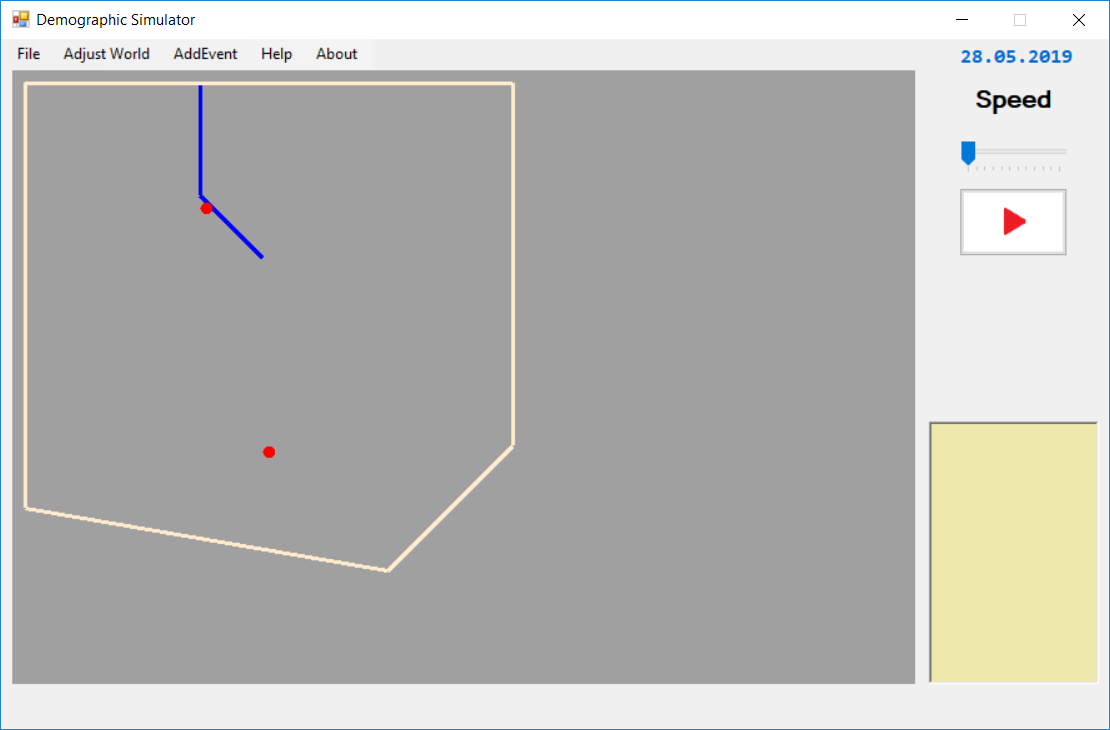
\includegraphics[width=\textwidth]{main}  
  \caption{Okno główne}
  \label{fig:GUI1}
\end{figure}


Dodane zostały również dwa okna: generujące zdarzenia oraz zmieniające parametry mapy, których wstępna wizualizacja nie została przedstawiona w specyfikacjach, a same klasy zostały pominięte w modelu UML.

\begin{figure}[H]
    \centering
    \begin{subfigure}[b]{0.49\textwidth}
        \centering
        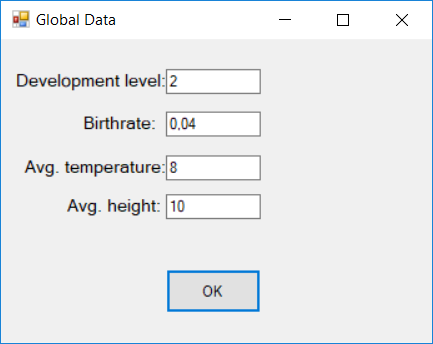
\includegraphics[width=1\textwidth]{adjust}
        \caption{Dostosowanie mapy}
    \end{subfigure}
    \begin{subfigure}[b]{0.49\textwidth}
        \centering
        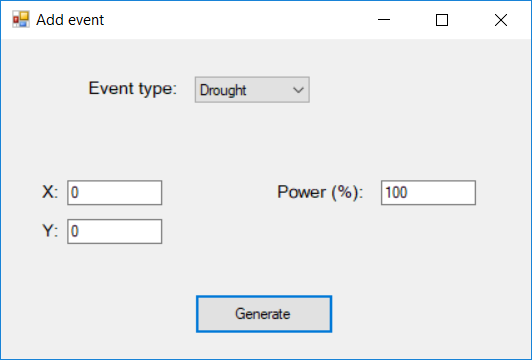
\includegraphics[width=1\textwidth]{event}
        \caption{Dodawanie zdarzeń}
    \end{subfigure}

    \caption{Okna pomocnicze}
    \label{fig:GUI2}
\end{figure}

\subsection{Plik wejściowy}

\tab Zmiany w dostarczanym pliku wejściowym ograniczyły się do zrezygnowania z podawania oddzielnej temperatury do każdego z miast -- opcjonalnym argumentem przy wprowadzaniu miast pozostała wysokość. Dodatkowo, zmieniono nazwy parametrów globalnych: 
\begin{itemize}
\item zamiast temperatura\_globalna należy podać srednia\_temperatura,
\item zamiast wysokosc\_globalna należy podać srednia\_wysokosc.
\end{itemize}

\subsection{Sytuacje wyjątkowe}

\tab Do sytuacji wyjątkowych zostały dodane ograniczenia planszy -- parametry muszą się zawierać w obszarze mapy, gdzie X ma być mniejszy niż 600, a Y mniejszy niż 500. Ponadto, program uniemożliwi podania współczynnika rozwoju cywilizacyjnego powyżej 10, przyjętego za maksymalną wartość tego parametru.

\section{Zmiany względem projektu aplikacji}

\tab Wiele metod umieszczonych na diagramie klas zmieniło parametry bądź też zwracane typy. Do najistotniejszych przykładów można zaliczyć:

\begin{itemize}
\item Metoda interfejsu \textit{IGameEvent} o nazwie \textit{ProceedEvent} zmieniła się na typ void, uzyskała także parametry w postaci punktu centralnego i mocy (liczby całkowitej od 0 do 100). Metoda oddaje także parametry referencyjne z liczbą ofiar i/lub migrantów.
\item Metoda \textit{MakeTimeJump} nie przyjmuje już liczby miesięcy do przesunięcia czasowego, a zawsze wykonuje przeskok jednego miesiąca.
\end{itemize}

\tab Powstały także nowe metody, upraszczające inne metody, które były bardziej złożone. Przykładem takiego podziału jest \textit{ReadData}, z którego zostały wydzielone metody do odczytu poszczególnych linii pliku konfiguracyjnego.

\section{Działanie programu}

\tab Uruchomienie programu powoduje otwarcie głównego okna programu, przedstawionego w poprzedniej sekcji. Wygląd okna będzie jednak neutralny, dopóki nie zostanie wczytany poprawny plik konfiguracyjny:

\begin{figure}[H]
  \centering
  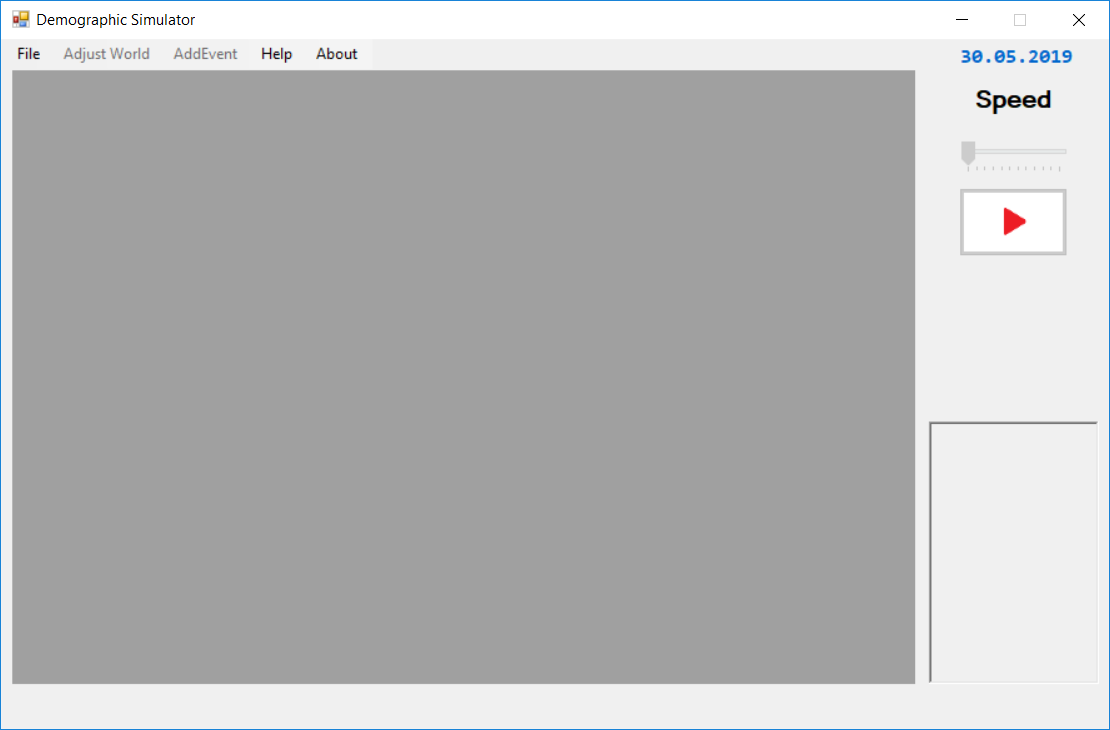
\includegraphics[width=\textwidth]{offline}  
  \caption{Okno aplikacji przed uruchomieniem symulatora}
  \label{fig:off}
\end{figure}

\tab Można tego dokonać wybierając opcję \textit{Load file} z menu \textit{File}. W przypadku podania niewłaściwego pliku lub pliku z niepoprawnymi wartościami program wypisze na ekranie stosowny komunikat do zaistniałej sytuacji, wskazując na źródło błędu, a w przypadku pojedynczych błędów w linijkach pliku także numery błędnych linii.

Czerwony przycisk start rozpoczyna działanie symulacji. Można kontrolować jej przebieg za pomocą znajdującego się nad nim suwaka. W przypadku wygenerowania zdarzenia program wyświetli komunikat z informacjami o zdarzeniu.

\begin{figure}[H]
  \centering
  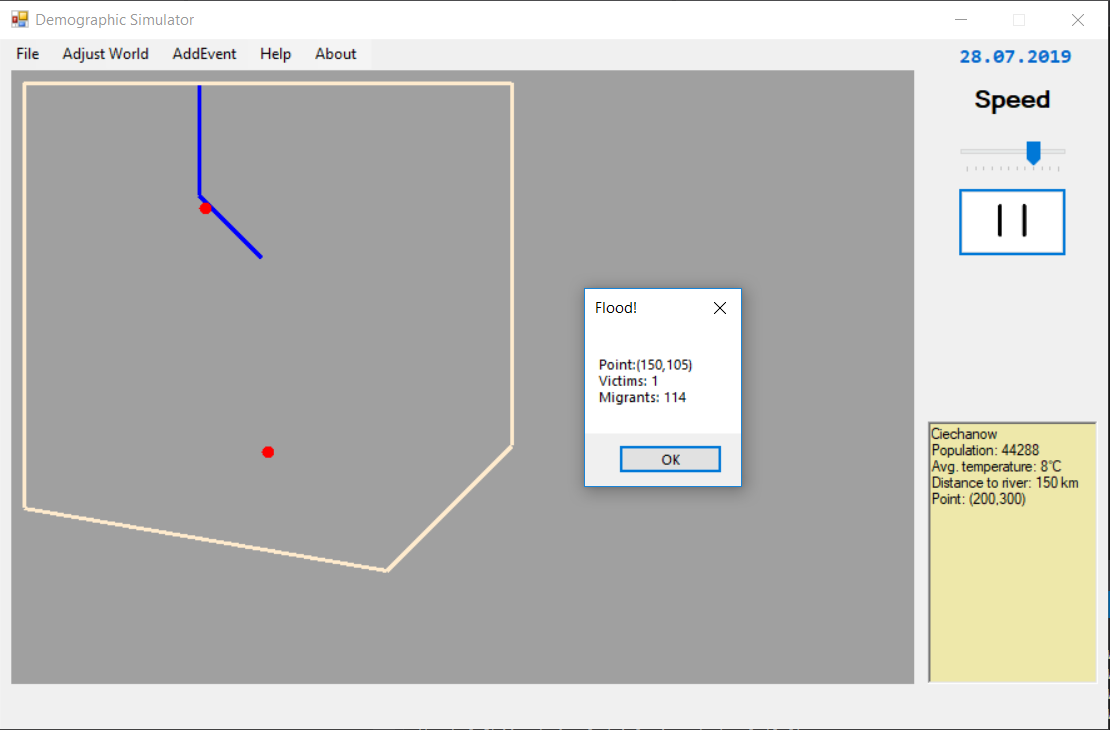
\includegraphics[width=\textwidth]{evt}
  \caption{Zdarzenie wywołane przez program}
  \label{fig:evt}
\end{figure}

\tab Symulacja zostanie wznowiona po zamknięciu wyskakującego okna. Dla ułatwienia kontroli, możliwe jest użycie przycisku pauzy także w momencie odczytu wydarzenia, żeby uniemożliwić programowi generowanie kolejnych wydarzeń.

Użytkownik może poza symulacją lub w trakcie symulacji zmieniać parametry lub dodawać zdarzenia ręcznie za pomocą przycisków znajdujących się na górnym menu. Wywołują one okna opisane w poprzedniej sekcji.

Program może w dowolnym momencie zamknąć aplikację lub wczytać kolejny plik do symulacji -- program w razie potrzeby zamknie samodzielnie wątki związane z poprzednią symulacją, przygotowując się do kolejnej.

\section{Podsumowanie i wnioski}

\subsection{Założenia, które udało się spełnić}

\tab Kluczowym założeniem projektu indywidualnego było zapoznanie się z nowym językiem programowania. Dlatego przy planowaniu aplikacji starałem się ułożyć taki model oprogramowania, który umożliwi wykorzystanie wielu rozwiązań programistycznych, z którymi spotkałem się wcześniej w większym lub mniejszym stopniu, w danym projekcie. Do takich rozwiązań należały między innymi:
\begin{itemize}
\item wielowątkowość,
\item przeciążanie metod i operatorów,
\item zastosowanie interfejsów,
\item obsługa zdarzeń.
\end{itemize}
\tab Większość z nich znalazła zastosowanie w programie, innych rozwiązań nauczyłem się w trakcie rozwiązywania problemów. Przykładem takich rozwiązań mogą być parametry referencyjne metod, które umożliwiają na proste uzyskanie kilku konkretnych informacji z metody bez potrzeby tworzenia dodatkowych klas.

\tab Projekt został także w pełni zrealizowany pod względem dokumentacji. Wszystkie dokumenty założone na początku jako produkty projektu zostały przygotowane i oddane. 

\subsection{Założenia, które nie zostały w pełni spełnione}

\tab Zapoznanie się z językiem programowania przy budowie pojedynczej aplikacji wiązało się z pewnymi ograniczeniami. Nie wszystkie mechanizmy charakterystyczne dla języka C\# zostały w nim wykorzystane, z uwagi na upływający czas lub nieznalezienie dla nich zastosowania w danym projekcie. Są to między innymi:

\begin{itemize}
\item synchroniczna praca wątków,
\item alternatywne wyrażenia (np. Lambda).
\end{itemize}

\tab Innym problemem, który został zrealizowany, jednak w sposób odmienny od tego założonego na początku, były wyliczenia symulacyjne. Pierwotnie miały one być oparte bezpośrednio na analizie prostych danych statystycznych (takich jak średnie/maksymalne wartości wysokości, temperatur). Jednak przy ilości i złożoności tych zagadnień odbiegających od pierwotnej roli programu zdecydowałem się wyważyć te zdarzenia na podstawie testów, żeby uzyskać czytelne w programie i satysfakcjonujące symulacje na podstawie niewielkiej ilości danych. Skutkiem tej decyzji jest duża ilość liczb w programie, które nie są wprost opisane żadnymi demograficznymi właściwościami.

\subsection{Wnioski}

\begin{enumerate}
\item Język C\# okazał się być bardzo ciekawym językiem programowania, pełnym rozwiązań niedostępnych w innych językach obiektowych, takich jak np. Java. Wiedza o tym języku wyniesiona z tego projektu może być znaczącym czynnikiem dla ukończenia studiów czy też znalezienia przyszłej pracy.

\item Sam koncept symulacji demograficznej był problemem bardzo złożonym i na potrzeby realizacji projektu musiałem przyjąć pewien poziom abstrakcji. Dlatego złożone i skomplikowane zdarzenia naturalne zostały zdefiniowane prostymi zależnościami oraz wartościami losowymi. Najważniejszy koncept tego problemu został zrealizowany -- wzrost pewnych wartości powoduje faktyczne zwiększenie prawdopodobieństwa powiązanych z nim wydarzeń. Bardzo istotne było dla mnie umożliwienie samodzielnego funkcjonowania (,,życia'') miast przedstawionych na mapie, co zostało zrealizowane.

\item Utworzony symulator może stanowić bazę dla przyszłych projektów. Wiele mechanizmów zastosowanych w projekcie może znaleźć zastosowanie np. w prostych grach strategicznych.
\end{enumerate}

\begin{center}
\begin{tabular}{ |c|c|c|c|c| } 
 \hline
 \textbf{Data:} & \textbf{Autor:} & \textbf{Zakres:} & \textbf{Zatwierdził:} & \textbf{Wersja:} \\ 
 \hline
 28.05.2019 & MS & Utworzenie dokumentu, wstęp & MS & 0.1 \\ 
 \hline
 28.05.2019 & MS & Opis zmian & MS & 0.2 \\ 
 \hline
 30.05.2019 & MS & Prezentacja działania programu & MS & 0.3 \\ 
 \hline
 30.05.2019 & MS & Sformułowanie podsumowania i wniosków & MS & 1.0 \\ 
 \hline
 \end{tabular}
\end{center}

\end{document}
